
\subsection{PAH band ratios}
\label{sect:pah_ratios}

Both the 6.2 and 7.7~$\mu$m features are thought to be coming from ionized PAHs and the 11.2~$\mu$m feature from neutral PAHs. Therefore we expect to see a correlation between the intensities of 6.2 and 7.7~$\mu$m PAH features normalized by the 11.2~$\mu$m feature.  Figure \ref{PAHlines}  compares the PAH flux ratios of 7.7/11.2  and 6.2/11.2 features. The figure shows a good correlation between these two PAH line ratios, consistent with that of the SINGS sample shown by \citet{Smith:2007lr}.
A similar correlation was also reported by  \citet{Galliano2008} for a sample of galaxies and a handful of extended H{\sc ii} regions
and by \citet{Vermeij2002} for Galactic and Magellanic Cloud H{\sc ii}\,regions. This provides evidence that the PAH emission from M31 is not unusual. 


\begin{figure}
\centering
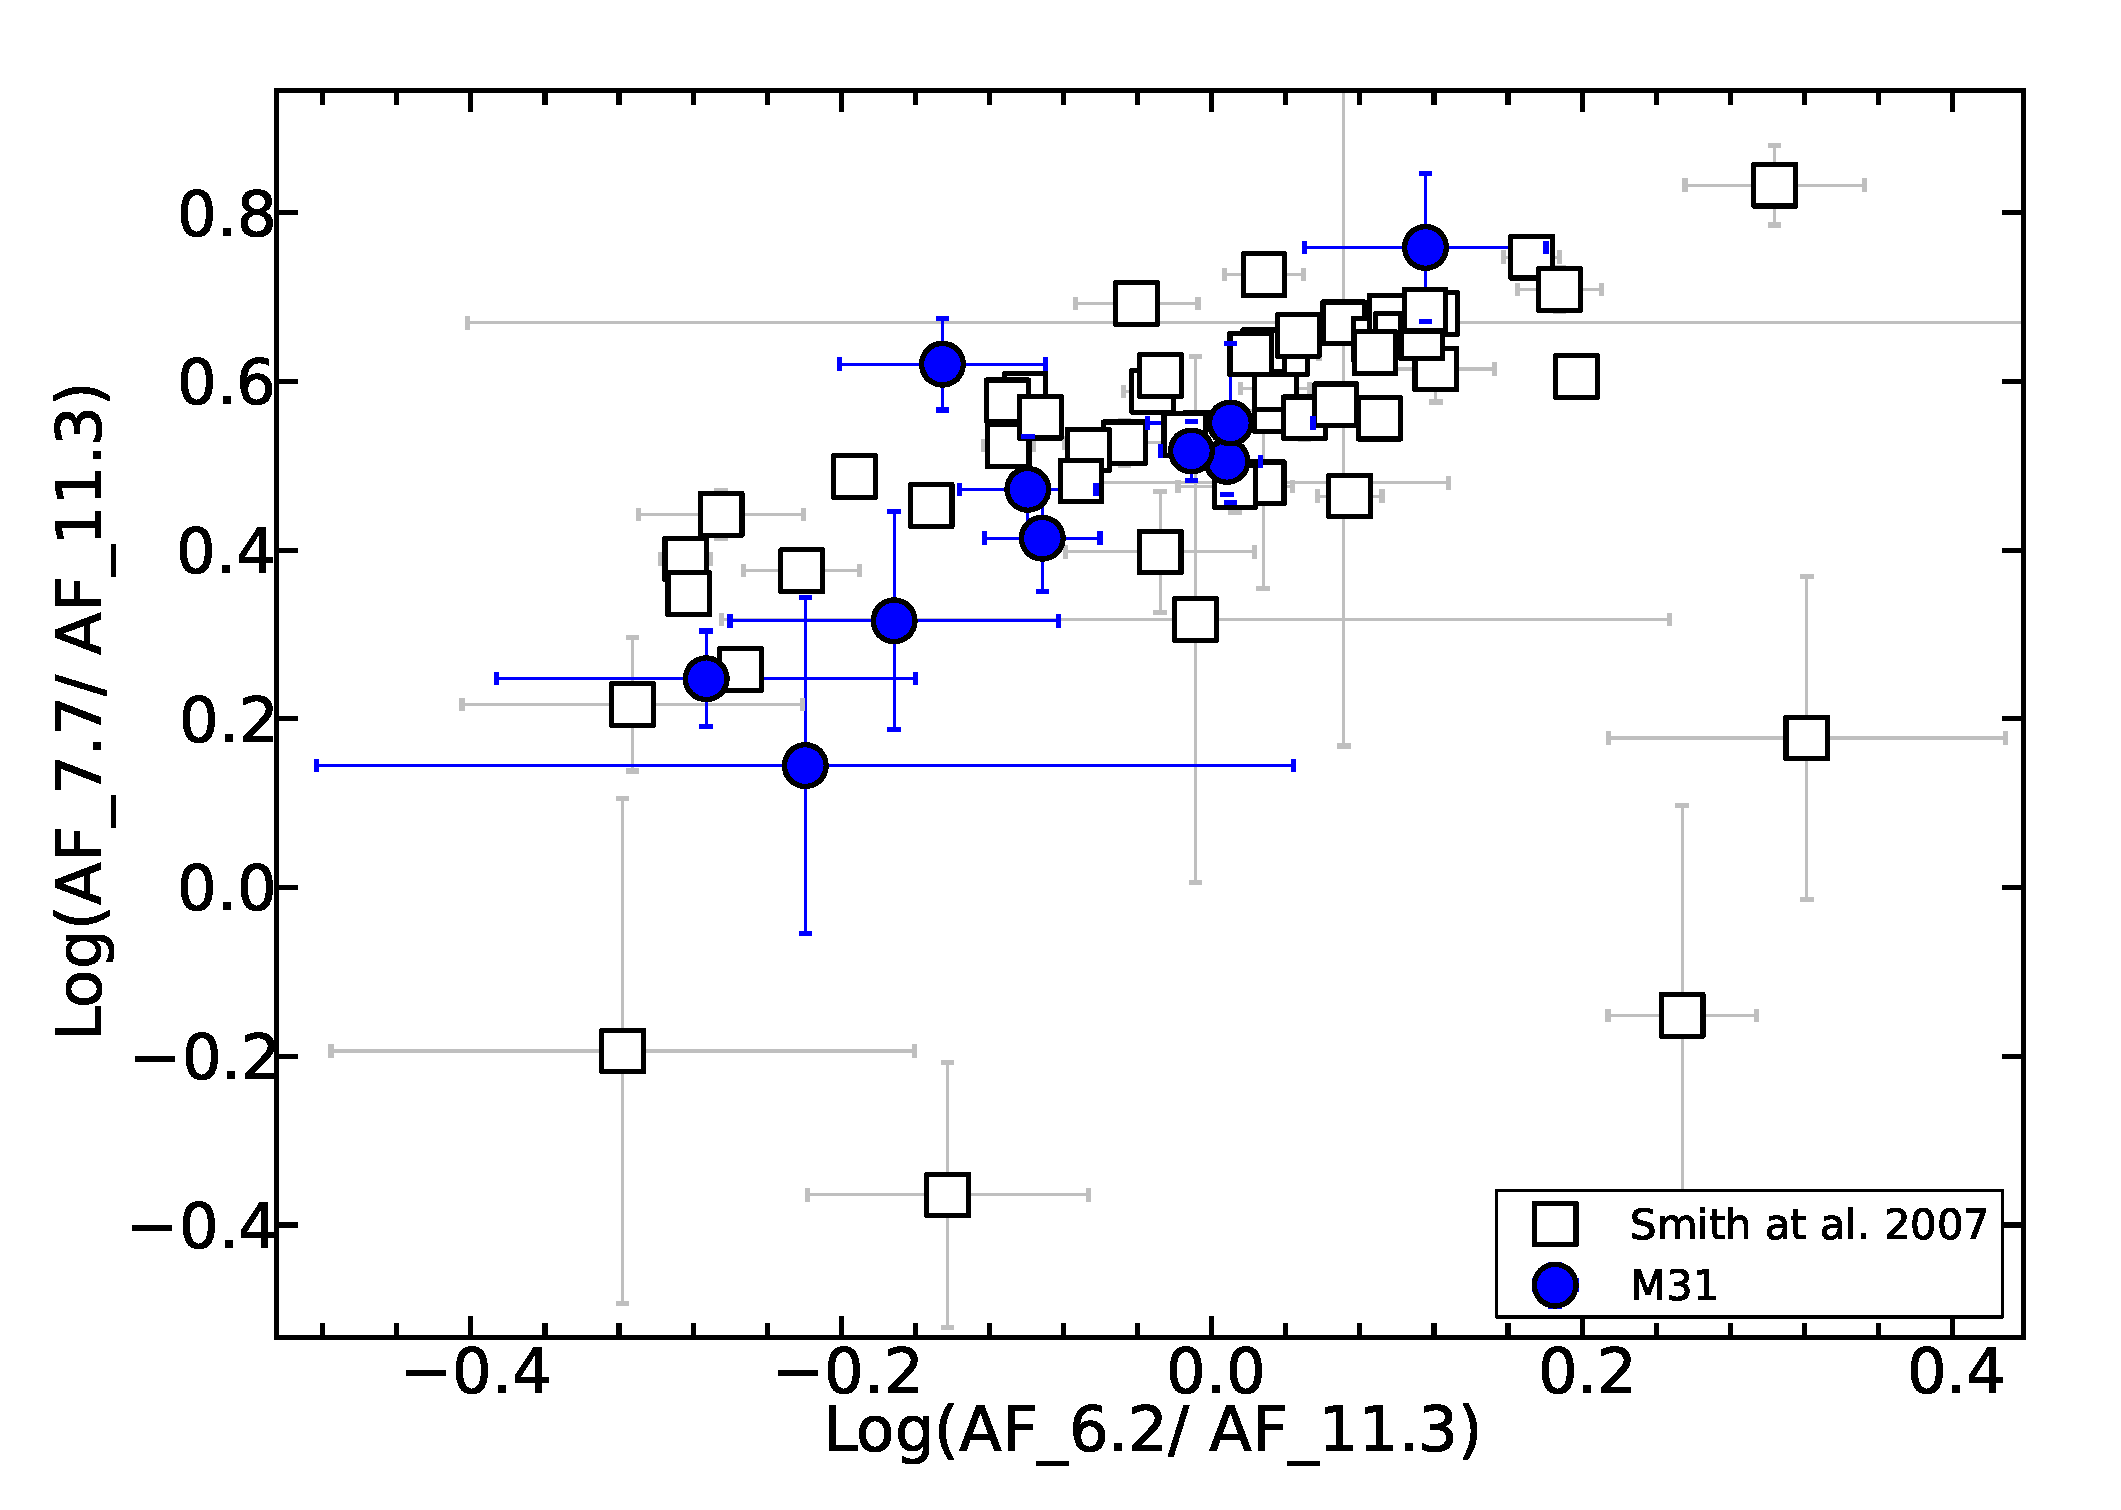
\includegraphics[scale = 0.4]{./fig8.eps}
\caption{Ratios of PAH feature fluxes (7.7~$\mu$m/11.2~$\mu$m versus 6.2~$\mu$m/11.2~$\mu$m) for 10 regions in M31.
Open squares represent the central regions of nearby galaxies as observed in the SINGS sample by \citet{Smith:2007lr}.
}
\label{PAHlines}
\end{figure}


\begin{figure*}
\centering
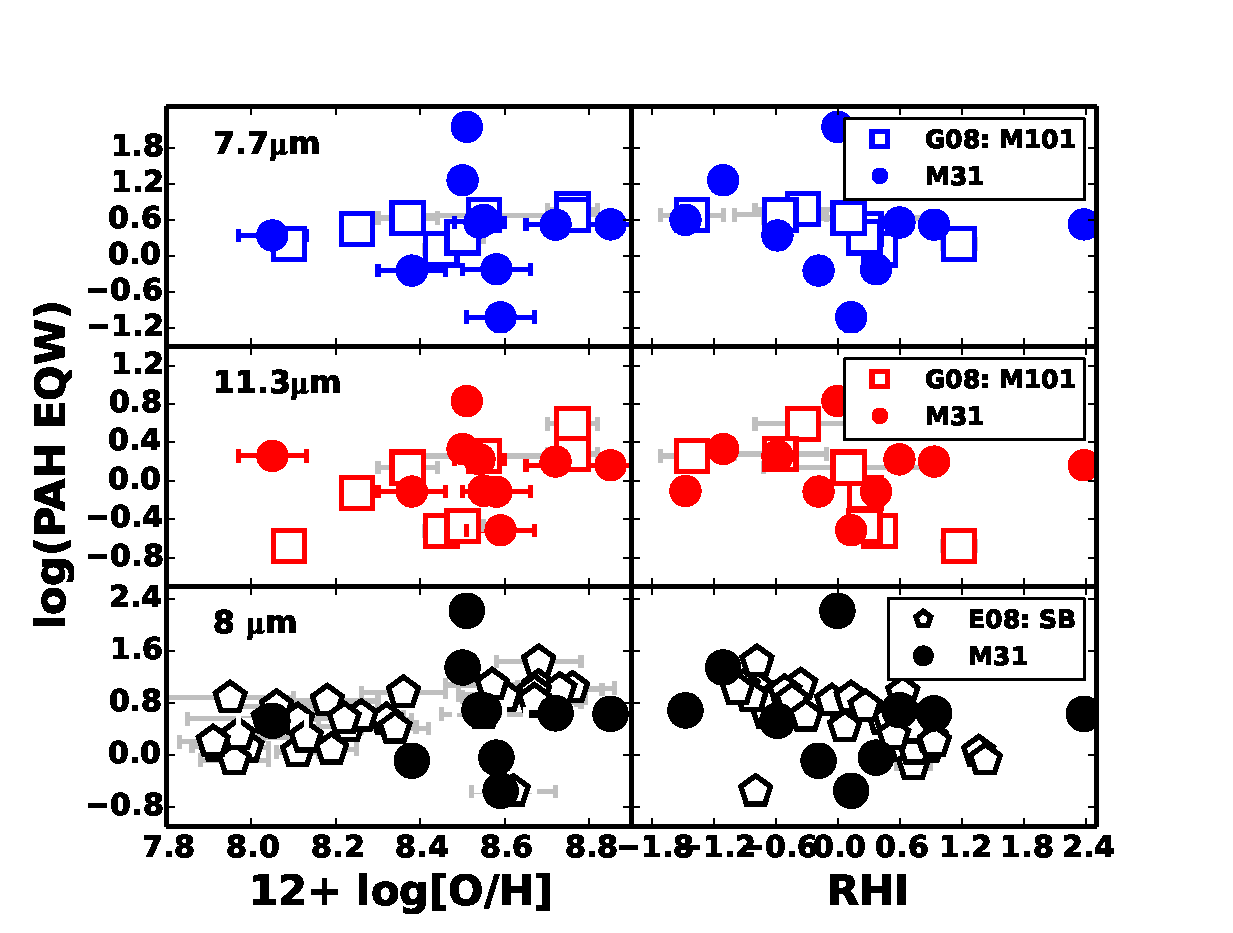
\includegraphics[scale=0.85]{./fig9.eps}
\caption{Equivalent width of  PAH feature versus metallicity (left panels) and radiation hardness index (RHI; right panels).
Equivalent  widths are not normalized; metallicities of the M31 regions have had 0.35~dex subtracted to account for the offset  between direct and strong-line measurements \citep{Croley2015}. 
Solid points: M31 sample; triangles represent upper limits. Open points:  starburst galaxy sample from \citet[bottom panels]{Engelbracht_2008} or
 H~{\sc ii} regions in M101 observed  by \citet[middle and top panels]{Gordon:2008lr}.  
}
\label{rhi_met_eqw}
\end{figure*}


\subsection{PAH equivalent widths versus radiation hardness and metallicity}
\label{sect:eqw_rh}

As mentioned in the introduction, PAH equivalent widths tend to decrease as radiation hardness increases,
and as metallicity decreases \citep{Calzetti:2010fk}.  

Figure~\ref{rhi_met_eqw} shows the equivalent widths of the  8~$\mu$m feature 
(a combination of the 7.7, 8.3 and 8.6~$\mu$m PAHFIT components) and the 
 7.7 and 11.2~$\mu$m features as a function of both metallicity and RHI. The starburst galaxy sample of \citet{Engelbracht_2008} 
and  H{\sc ii} regions in M101 \citep{Gordon:2008lr} are plotted for comparison.
The M31 regions cover approximately the same range of measurements as the starburst galaxies and M101 H{\sc ii} regions;
the outliers are regions 3 and 9 with high equivalent widths (uncertain due to low continuum, see Section~\ref{sect:pahfit}) and
region 8 with low equivalent widths (noisy spectrum as well as substantial modelled contribution from starlight, see Figure~\ref{PAHFITplots}).
No clear trend is defined by the M31 data, unsurprising given the uncertainties and the limited
number  of regions.
We do not have enough data from low-metallicity regions in M31 to observe the expected decrease of PAH EQW with decreasing 
metallicity; however the M31 data occupy the same region of parameter space as the M101 data
and we conclude that the EQWs of the regions in M31 are consistent with previously published ``normal'' values.



